\section*{Resampling}
We present two resampling strategies in this section. The overall goal
of all resampling methods is to remove particles with negligible
weights with a high probability and replicate those with high
weights. After resampling, the future particles are more concentrated
in domains of higher posterior probability, which entails improved
estimates. It can, of course, happen that a particle with a low weight
at time $k$ has a high weight at time $k+1$, in which case resampling
could be wasteful. It should also be mentioned that if particles have
(unnormalised) weights with a small variance, resampling might be
unnecessary. This is discussed briefly at the end of this section.

As above, we denote by $\{ x^{(i)}; w^{(i)} \}_{1 \le i \le N}$ the
set of particles with their associated weights at some time $k$ (which
is omitted in the notation). We assume that the weights have already
been normalised such that $\sum_i w^{(i)} = 1$. We further denote by
$\{ \tilde{x}^{(i)}; \tilde{w}^{(i)} \}_{1 \le i \le N}$ the particles
and weights after resampling took place. We require the particles
$\tilde{x}^{(i)}$ to be weighted equally which implies, since we also
require the weights to be normalised that $\tilde{w}^{(i)} = 1/N$.

The use of resampling to improve importance sampling was originally
introduced by Gordon, Salmond and Smith in~\cite{gordon}. The
resampling methods presented here are two of the most popular amongst
the literature, see~\cite{douc}. The most simple resampling strategy,
called \emph{multinomial resampling} is not discussed here due to its
poor performance compared to other techniques. It is mentioned because
it is the method introduced in~\cite{gordon} as part of the\emph{
  bootstrap filter} that uses the prior as the proposal density
(cf.\ Examples~\ref{ex:1} and~\ref{ex:lv1}).

Both methods presented in the following are based on drawing samples
from the point mass distribution
$\sum_{j=1}^N w^{(j)} \delta_{X^{(j)}}$. In practice, this is achieved
by repeated uses of the inversion method, which itself uses the
empirical cumulative distribution function (cdf) associated with the
weights. This is based on the following fact:

\textbf{Claim.}\quad If $U$ is a uniform random variable on $(0,1]$
then $X = F^{-1}(U)$ has distribution $F$, where $F$ is the cdf of $X$
and $F^{-1}(t) = \min \{ x \mid F(x) = t \}$ is the inverse cdf.

\textbf{Proof.}\quad Let $U \sim \mathcal{U} (0,1]$. Then
\begin{align*}
  P(F^{-1}(U) \le x) &= P(\min \{x \mid F(x) = U \} \le x ) && \text{(definition of $F^{-1}$)} \\
                     &= P(U \le F(x)) \\
                     &= F(x) && \text{(definition of distribution of $U$)}\,.
\end{align*}
\hfill$\square$

The inversion method can be explained visually as follows. We plot the
empirical cdf of the weights and sample from
$U \sim \mathcal{U}(0,1]$. We denote the actual value of the sample by
$u$. We then draw a horizontal line from the coordinate $(0,u)$ to the
right until it intersects one of the bars, see
Figure~\ref{fig:ecdf}. The index of the bar that is intersected
determines the new sample.

\begin{figure}
  \centering 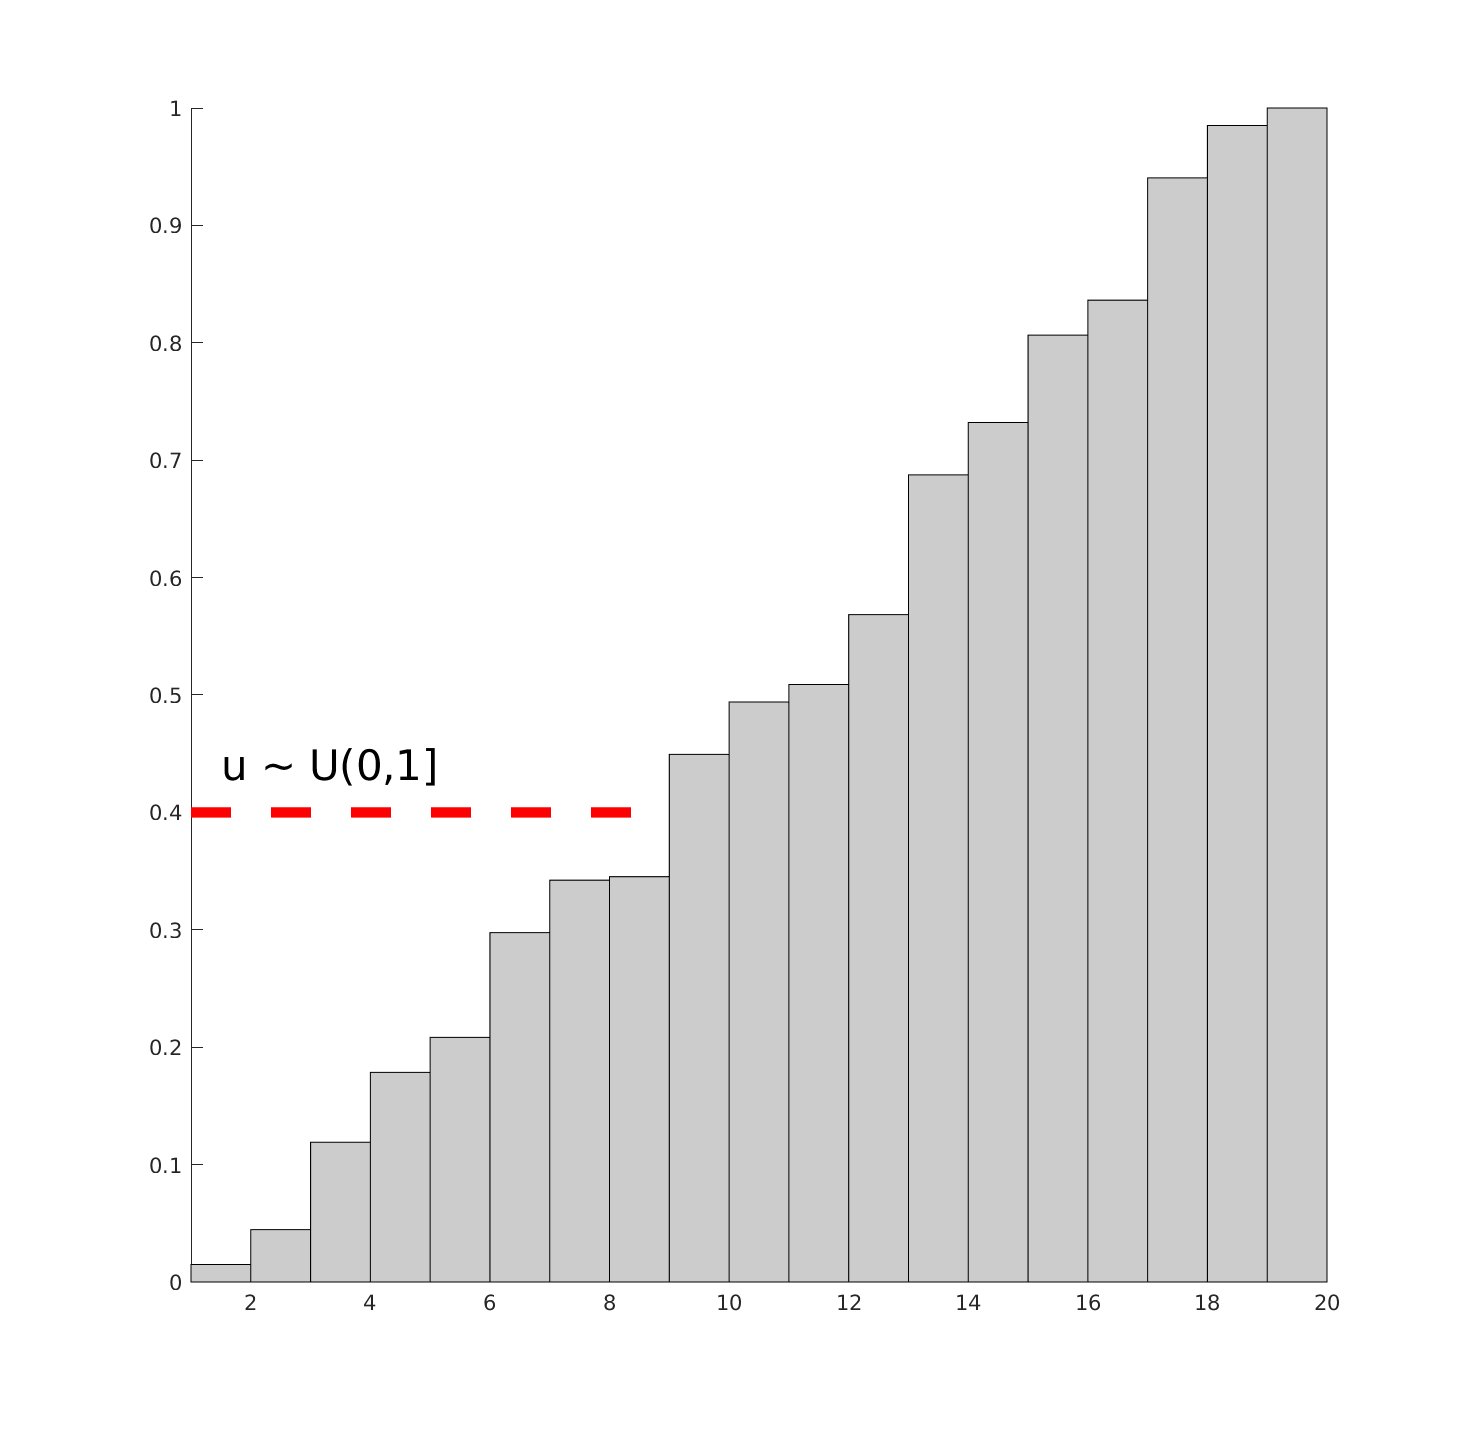
\includegraphics[width=0.5\textwidth]{figures/ecdf.png}
  \caption{Visualisation of the inversion method. The bars represent
    the empirical cumulative distribution function associated with a
    set of 19 weights. The dashed line is horizontally drawn from the
    value of $u$ at the vertical axis until it ``hits'' a bar. The
    index of the bar yields the generated sample (in this case the new
    sample is therefore 9). }
  \label{fig:ecdf}
\end{figure}

In our case, we do not draw just one sample $U$ but we generate $N$
different samples $\{U_i\}_{1 \le i \le N}$ in such a way that they
are sorted in ascending order. For every of these samples (from lowest
to highest) we look for the intersected bar and add its index to a
list. This list then corresponds to the indices of the particles that
should be resampled. Consider the following example: Suppose we had
five particles and the list of indices after the resampling reads
$\{1,3,4,4,5\}$. Then, particles $X^{(1)},X^{(3)},X^{(5)}$ should be
resampled, particle $X^{(4)}$ should even be duplicated. Particle
$X^{(2)}$, however, will be dropped. In other words, the particles
after the resampling are
\begin{gather*}
  \tilde{X}^{(1)}=X^{(1)},\ \tilde{X}^{(2)}=X^{(3)},\ \tilde{X}^{(3)}=X^{(4)},\\
  \tilde{X}^{(4)}=X^{(4)},\ \tilde{X}^{(5)}=X^{(5)}\,.
\end{gather*}

The two strategies presented in the following only differ in the way
the $U_i$s are generated. We summarise the results in
Algorithm~\ref{alg:resampling}.

\begin{algorithm}[htpb]
  \SetAlgoLined
  \KwData{$N$ samples $U_i \sim \mathcal{U}(0, 1]$ sorted in ascending order;\
    list of weights}
  \KwResult{List of indices $I$ that represent that particles to be resampled}
  $C$ = \texttt{cumsum}(weights) \tcp*{Generate the empirical cdf as list of
    accumulated sums\footnotemark}
  $I$ = zeros(N)\;
  $i,j = 0$\;
  \While{$i < N$}{
    \eIf(\tcp*[h]{Found intersecting bar}){
      $U_i < C_j$
    }{
      $I_i = j$\;
      $i = i+1$\;
    } {
      $j = j + 1$\;
    } }
  \caption{Resampling using the empirical cdf}\label{alg:resampling}
\end{algorithm}

\subsection*{Systematic Resampling}
This algorithm separates the sample space into $N$ divisions. One
random offset, drawn from a $\mathcal{U}[0, 1)$ distribution, is used
to choose where to sample from for all divisions. This guarantees that
every sample is exactly $1/N$ apart.

In other words, the $U_i$s are generated by sampling
$\tilde{U} \sim \mathcal{U}[0, 1)$ and defining
\[
  U_i = \frac{\tilde{U} + i-1}{N} \quad \text{for } i = 1, \dotsc, N
  \,.
\]

\subsection*{Stratified Resampling}
\footnotetext{Here, the function \texttt{cumsum} is assumed to work in
  the same way as, for example, MATLAB's or NumPy's \texttt{cumsum}
  function. That is, \texttt{cumsum([1,2,3,4])} should return
  \texttt{[1,3,6,10]}.}  This algorithm is similar to the previous
one, its aim is to make selections relatively uniformly across the
particles. We start by partitioning the $(0,1]$ interval into $N$
disjoint sets,
$(0,1] = (0, 1/N] \cup (1/N, 2/N] \cup \dotsm \cup ((N-1)/N, 1]$. The
$U_i$s are then drawn independently in each of the sub-intervals:
\[
  U_i \sim \mathcal{U}((i-1)/N, i/N]\,.
\]

We mentioned earlier that resampling might be unnecessary if the
weights are sufficiently uniform and we would like to have a criterion
allowing us to check whether resampling should be performed. To that
end the effective sampling size ($ESS$) is often used which can be
estimated using
\begin{equation}
  \label{eq:ESS}
  ESS \approx {\left( \sum_{i=1}^N {\left( w_t^{(i)} \right)}^2
    \right)}^{-1} \,.
\end{equation}
For more details, see~\cite[179]{arulampalam}. If the variance of the
weights is maximal, \ie, if all but one of the weights are zero, the
value of $ESS$ is 1. If, however, the weights all have the same value
$w_t^{(i)} = 1/N$ the value of $ESS$ is $N$, since
\[
  {\left( \sum_{i=1}^N {\left( \frac{1}{N} \right)}^2 \right)}^{-1} =
  {\left( N \frac{1}{N^2} \right)}^{-1} = N \,.
\]
Therefore, we will only resample if $ESS$ is below a certain
threshold, e.\,g.\ $N/2$.

We have now gathered everything we need to implement a particle
filter, since essentially particle filters are simply a combination of
sequential importance sampling and one of the resampling strategies
(or, of course, any other resampling algorithm not presented
here). Consequently, these methods are sometimes called
\emph{Sequential Importance Sampling with Resampling} abbreviated by
SIR or SIS/R. Other popular names include \emph{Bootstrap filter},
\emph{Monte Carlo filter}, \emph{Survival of the fittest} or
\emph{Condensation algorithm}.

%%% Local Variables:
%%% mode: latex
%%% TeX-master: "../main"
%%% End:
